\section{Methodology}

In this section, we provide a detailed introduction to our proposed MTransLLAMA framework, which efficiently transfers the image-based LMM to handle video understanding tasks. It preserves the extensive pre-training knowledge of the image-text model, resulting in improved transfer generalization. MTransLLAMA achieves early multi-modal fusion and temporal-spatial cyclic fusion by reusing the image-text model. To endow the image-text model with the ability to understand temporal information and reduce video pre-training costs, MTransLLAMA proposes a channel swapping method that reuses multi-modal attention module parameters in the image-text model (detailed in Section \ref{section3.2} and Section \ref{section3.3}). 
% For better transfer of data attention interaction information, 
To better capture local and global semantics of data,
MTransLLAMA introduces a spatial-temporal domain dynamic routing transfer for multiple modalities (discussed in Section \ref{Section3.4}).

\subsection{Overview of MTransLLAMA}
% Problem statement

Given the context $\mathbf{C}$ (including dialogues, instructions, questions, etc.) and the corresponding video $\mathbf{v} \in \mathbb{R}^{T \times 3 \times H \times W}$ comprising $T$ frames sampled from the video sequence, each of size $H \times W$, our proposed MTransLLAMA aims to transfer an image-based LMM to generate answers $\mathbf{C}_o$ in natural language form with the combination of video and text. 
% Overview of the framework
% To efficiently transfer a pre-trained image-text LLM to a video-text LLM, we propose MTransLLAMA, which 
The proposed MTransLLAMA has three key components, including a multi-modal spatial-temporal early fusion module, a multi-modal query temporal reusing module, and a dynamic attention routing module. The goal of each module is briefly described as follows.

\subsubsection{Multi-modal Spatial-temporal Early Fusion}
Traditional video-based LMMs usually adopt the following mechanism for question answering (QA), \textit{i.e.},
\begin{equation}
\label{eq:traditional fusion}
    \mathbf{C}_o = \text{LLM}(\mathbf{E}_t, f_{\mathbf{\theta}}(\mathbf{E}_v,\mathbf{q})),
\end{equation}
where $\mathbf{C}_o$ is the answer generated by LLM; $f_{\mathbf{\theta}}$ is the spatial-temporal module with learnable parameters $\mathbf{\theta}$; $\mathbf{E}_t$, $\mathbf{E}_v$ and $\mathbf{q}$ are text embeddings, visual embeddings and learnable queries, respectively. 
Unlike the conventional methods, our proposed fusion mechanism extracts the spatial-temporal information of the dialogue and instruction from early layers and interacts with visual features, which can be formulated as follows,
\begin{equation}
\label{eq:our fusion}
    \mathbf{C}_o = \text{LLM}(\mathbf{E}_t, f_{\mathbf{\theta}}(\mathbf{E}_t, \mathbf{E}_v, \mathbf{q})),
\end{equation}
Besides, as shown in Fig.~\ref{fig:intro}, traditional video-based LMMs place the temporal model modules entirely after the spatial model modules. However, the output of the spatial models consists of high-level visual features, which lack the interaction of low-level spatial-temporal information. Our method iteratively cycles through spatial and temporal modules, accomplishing the spatial-temporal fusion of multi-modal information at various granularities.

\subsubsection{Multi-modal Query Temporal Reusing}
For LLM-based video understanding methods~\cite{zhang2023video,maaz2023video} that deal with temporal information, a separately trained temporal modeling module is typically required. However, pre-training temporal modules consumes vast data and computational resources, making it unaffordable to learn $f_{\theta}$ in downstream video understanding tasks. Additionally, the video pre-training phase might compromise the rich image-text information, leading to a reduction in transferability. To address the above challenge, our innovative strategy involves reusing the pre-trained self-attention layers in multi-modal models for temporal modeling. Interestingly, we find the pre-trained spatial self-attention weights can work well for temporal modeling with efficient low-rank adaptation (LoRA). In addition, we adopt a channel swapping strategy to further reduce the cost of temporal modeling. 

\subsubsection{Dynamic Attention Routing}
Existing research~\cite{zhou2021trar,tian-etal-2023-dynamic} shows that in certain vision and language tasks, multi-modal reasoning often requires visual attention from different receptive fields. To enable the model to understand both the high-level semantics and local relations, we propose a dynamic attention routing (DAR) strategy in our designed multi-modal spatial-temporal model $f_{\theta}$. 
The router can automatically select cooperative attention masks. We not only perform dynamic routing on spatial attentions of the multi-modal data but also on temporal attentions.

\subsubsection{Training Loss}
% 把loss写在这里
During training, we aim for the LLM's output answer $\mathbf{C}_o$ to match our ground truth answer $\mathbf{C}_a$. We use the cross-entropy loss between the embedding token $G$ of the ground truth answer $\mathbf{C}_a$ and the probability distribution $\mathbf{p}$ of the output answer $\mathbf{C}_o$, following the same training process as all LLM workflows. The loss is shown as follows.
\begin{equation}
% \begin{split}
\label{eq:our fusion}
    \mathcal{L} = -\sum_{i} \mathbf{G}_i \log(\mathbf{p}_i),
    % G = \text{Tokenizer}(C_a)
% \end{split}
\end{equation}
where
\begin{equation}
% \begin{split}
\label{eq:our fusion}
    % L = -\sum_{i} G_i \log(p_i)\\
    \mathbf{G} = \text{Tokenizer}(\mathbf{C}_a),
% \end{split}
\end{equation}
and \text{Tokenizer} maps natural language to the output tokens of the LLM.

\subsection{Multi-modal Spatial-temporal Early Fusion}
\label{section3.2}
% 这个章节主要描述input和embedding，以及三组attention block，每组attention就简单用symbol表示出来即可

Given the context $\mathbf{C}$ and the corresponding video $\mathbf{v}$, we first extract the text and visual embeddings like BLIP-2. Text embeddings $\mathbf{E}_t \in \mathbb{R}^{K_T \times D}$ are derived from $\mathbf{C}$ using a Bert Tokenizer, where $D$ represents the embedding size, and $K_T$ denotes the sequence length after padding. 
The visual embedding $\mathbf{E}_v \in \mathbb{R}^{T \times K_V \times D}$ are obtained frame by frame using the Vision Transformer (ViT) as described by:
\begin{equation}
\label{eq:visual extract}
    \mathbf{E}_v =  \{ \mathbf{x}_{i}= \text{ViT}(\mathbf{v}_{i}) \mid \forall i = 1,...,T\}
\end{equation}
where $K_V$ is the number of tokens after encoding for each frame image.

Then, these video representations $\mathbf{E}_v$ are fed into the Q-former along with the queries $\mathbf{q} \in \mathbb{R}^{L \times D}$, and text embedding $\mathbf{E}_t$ for attention operations, allowing the multi-modal information to be represented by queries $\mathbf{q} \in \mathbb{R}^{T \times L \times D}$, where $L$ is the number of queries for each image.

At the first MTransLLAMA layer, we update the original multi-modal query $\mathbf{q}_0$ with spatial and temporal position embeddings as:
% \begin{equation}
% \label{eq3}
%     \mathbf{q}^0_{i,j} = \mathbf{q}_{j} + emb_t(i) + emb_s(j),
% \end{equation}
\begin{equation}
\label{eq3}
    \mathbf{q}^0_{i,l} = \mathbf{q}_{i,l} + \mathbf{e}^t_{i} + \mathbf{e}^s_{l},
\end{equation}
where $\mathbf{q}_{i,l}$ is the original query with sequence index $l \in (0,L)$ and the frame index $i$; and $\mathbf{e}^t$ and $\mathbf{e}^s$ are the learnable temporal and spatial positional embedding, respectively.

During the process of extracting video features, each layer of our feature extractor is composed of spatial self-attention, temporal self-attention, and cross-attention. By interacting text and image attention, we achieve the early fusion of text and visual embedding.

Due to the repetitive structure of the Q-former, we implement spatial-temporal recurrent feature extraction, which facilitates the interaction of spatial-temporal features at various granularities. This approach has been shown to be beneficial in previous research \cite{xiao2022video}.
\subsection{Multi-modal Query Temporal Reusing}
\label{section3.3}
% 这个章节主要描述channel swapping和LoRA以及三组attention的细节


\label{Section3.3}
\begin{figure}[!t]
    \centering
    \includegraphics[width=0.5\textwidth]{figs/reuse.pdf}
    \caption{Overview of Parameter Reuse: The temporal module is implemented by reusing the attention block parameters from the original Q-former, with small-parameter LoRA fine-tuning applied.}
    \label{fig:reuse}
\end{figure}

The reuse of pre-trained self-attention weights in the temporal modeling includes the channel swapping strategy and the efficient low-rank adaptation (LoRA), as shown in Fig.~\ref{fig:reuse}, which are demonstrated in this subsection in detail. 

\subsubsection{Channel Swapping}

We employ an image-text Q-former for video representation and a frozen projection layer to align with LLM Tokens. For a batch $B$ of data, we initially flatten $B$ and $T$ channels in queries, \textit{i.e.}, from $B \times T \times L \times D$ to $BT \times L \times D$ within each attention module of Q-former. This process allows the video representation to undergo spatial feature attention operations, enabling information interchange among different sequence number queries $j$ within a frame $i$ after they pass through cross-attention and self-attention in Q-former.

In the spatial attention module, we adopt self-attention, denoted as S-ATN, for query and text embeddings in the $m$-th layer, \textit{i.e.},
\begin{equation}
\label{eq4-1}
    {\mathbf{E}_t}^\prime,{\mathbf{q}}^\prime = \text{S-ATN}^L(\mathbf{E}_t \cup \mathbf{q}),
\end{equation}
where the superscript $L$ for $\text{S-ATN}^L$ denotes that the attention is across the $L$ dimension.
As shown in Fig.~\ref{fig:framework}, when interacting with visual embeddings, we calculate cross-attention, denoted as C-ATN, between visual embeddings and query embeddings, which can be formulated as follows,
\begin{equation}
\label{eq4-2}
    {\mathbf{q}}^\prime =\text{C-ATN}^L(\mathbf{E}_v, \mathbf{q}).
\end{equation}

% In the $m$-th layer, for frame $i$ from $0$ to $T$. We conduct self-attention or cross attention like:
% % \begin{equation}
% % \label{eq4}
% % \begin{split}
% %     {E_t(i,.)}^\prime,{q^m_{i,.}}^\prime = S\text{-}Self(E_t(i,.) \cup q^m_{i,.})\\
% %     {q^m_{i,.}}^\prime =S\text{-}Cross(E_v(i,.),q^m_{i,.})
% % \end{split}
% % \end{equation}
% \begin{equation}
% \label{eq4}
% \begin{split}
%     {E_t}^\prime,{q^m}^\prime = S\text{-}ATN^L(E_t \cup q^m)\\
%     {q^m}^\prime =C\text{-}ATN^L(E_v,q^m)
% \end{split}
% \end{equation}
% where S-Self represents the Spatial Self Attention Module and the S-Cross is the Spatial Self Attention Module.


In the temporal module, we reuse the parameters from the spatial attention module to reduce the cost.
% For temporal modeling, our Temporal-Attention module specifically reuses the parameters from Spatial-Attention to reduce cost of temoporal module. 
In this module, we reshape the batch data from $BT \times L \times D$ to $BL \times T \times D$ and calculate attentions across the $T$ dimension as follows, 
% In this module, the $B$ and $L$ channels in queries $B \times T \times L \times d$ are flattened to form $BL \times T \times d$. For queries with the same sequence number $j$ across different frames $i$, they possess similar semantic information. 
% We facilitate temporal attention information interchange between queries of the same sequence number but from different frames:
% \begin{equation}
% \label{eq5}
%     {q^m_{.,j}}^\prime = T\text{-}Self(q^m_{.,j})\\
% \end{equation}
\begin{equation}
\label{eq5}
    {\mathbf{q}}^\prime = \text{S-ATN}^T(\mathbf{q}),
\end{equation}
where $\text{S-ATN}^T$ represents the temporal self-attention operator.
% 这里再加几句话，说明这样做channel swapping的motivation和意义

The channel swapping can utilize temporal modeling and spatial modeling to handle the similarity of information, thereby efficiently processing video temporal information with minimal parameters.

\subsubsection{LoRA Fine-tuning}
To ensure that the new video representation is understandable by the frozen LLM, inspired by efficient fine-tuning techniques in NLP, we adopt a low-rank matrix adaptation (LoRA) approach for fine-tuning the Q and V matrices of the Query attention in Q-former while keeping all other parameters frozen:
\begin{equation}
\begin{split}
\label{eq6}
    \mathbf{W}_{qs} = \mathbf{W}_q + {LoRA}_s(\mathbf{W}_q)\\
    \mathbf{W}_{qt} = \mathbf{W}_q + {LoRA}_t(\mathbf{W}_q)
\end{split}
\end{equation}
where $\mathbf{W}$ is the weight of Q-former parameters. $s$ and $t$ represent the temporal and spatial attention layers, respectively.


\subsection{Dynamic Attention Routing (DAR)}

\label{Section3.4}
\begin{figure}[!t]
    \centering
    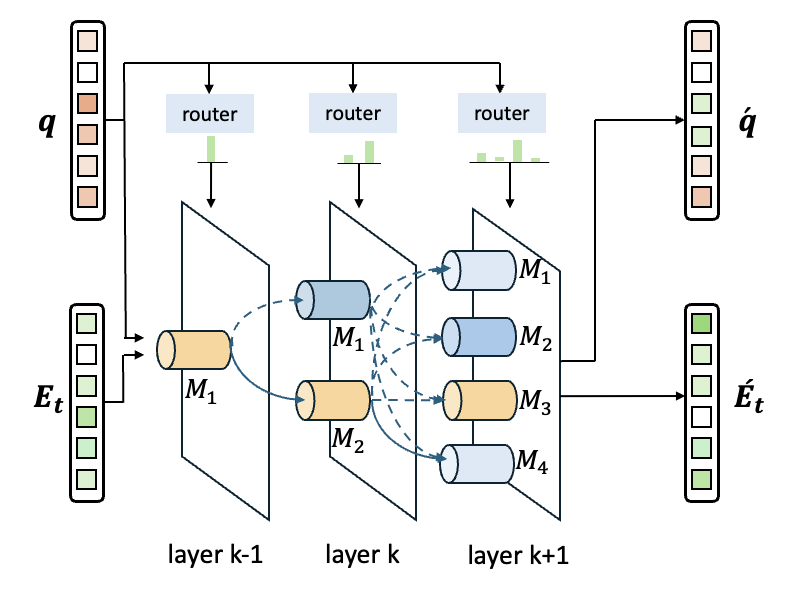
\includegraphics[width=0.5\textwidth]{figs/fig33.png}
    \caption{Overview of Dynamic Attention Routing: when using self-attention to fuse features between the text and the query, we apply masks $\mathbf{M}$ with different receptive fields to control the attention scope. As the attention progresses through layers, the selectable routing options increase, and the query is used to learn the routing probabilities $\alpha$ to choose the routing path}
    \label{fig:Dyn}
\end{figure}
As shown in Fig.~\ref{fig:Dyn}, in each self-attention layer, we introduce a dynamic attention routing (DAR), which is a new routing selection mechanism that enables the model to understand both the high-level semantics and local relations.
% To enable the model to understand both the overall semantics and local relations, our DAR introduces a new routing selection module in each self-attention layer. 
We initially design masks $\{\mathbf{M}_0,\dots, \mathbf{M}_l\}$ with different receptive fields to accommodate varying degrees of attention interaction. As the number of attention layers increases, we utilize more routing choices, simulating the modal inconsistencies of different semantic levels.

In the $k$-th attention layer, the router can route the cooperative attention masks group $\{\mathbf{M}_0,\dots,\mathbf{M}_{p_k-1}\}$, where $p_k$ is the number of mask matrices in the $k$-th layer of DAR. We average the attention weights with different masks using the routing layer to obtain the final representation after attention:
\begin{equation}
\label{eq10}
    DAR(\mathbf{q}) =\frac{[\mathbf{W}_q(\mathbf{E}_t \cup \mathbf{q})][\mathbf{W}_k(\mathbf{E}_t \cup \mathbf{q})]^T}{\sqrt{D_h}}\otimes\sum_{j=0}^{p_k-1}\alpha_j \mathbf{M}_j,
\end{equation}
where $\alpha$ is the routing probability. And $q_m$ is queries in the attention module. $\otimes$ represents the Hadamard product.

The routing probability $\alpha$ of the $k$-th attention layer can be obtained by conditional computation on the input. $\alpha$ can adjust the weighting of subsequent attention routing to achieve control over different receptive fields.
\begin{equation}
\label{eq11}
    \alpha = \text{MLP}(\text{APool}(\mathbf{q}))
\end{equation}
where APool(·) refers to the 1D adaptive average pooling performed over all the embeddings of patches in the image; and MLP is a two-layer multi-layer perceptron. 
% We keep all the parameters frozen except MLP during training.